\documentclass[14pt]{extreport}
\usepackage{gost}
\usepackage{hyperref}
\usepackage{makecell}
\usepackage{ragged2e}
\justifying


\renewcommand{\thefigure}{\arabic{figure}}
\renewcommand{\thetable}{\arabic{table}}


\begin{document}
\pagestyle{empty} 
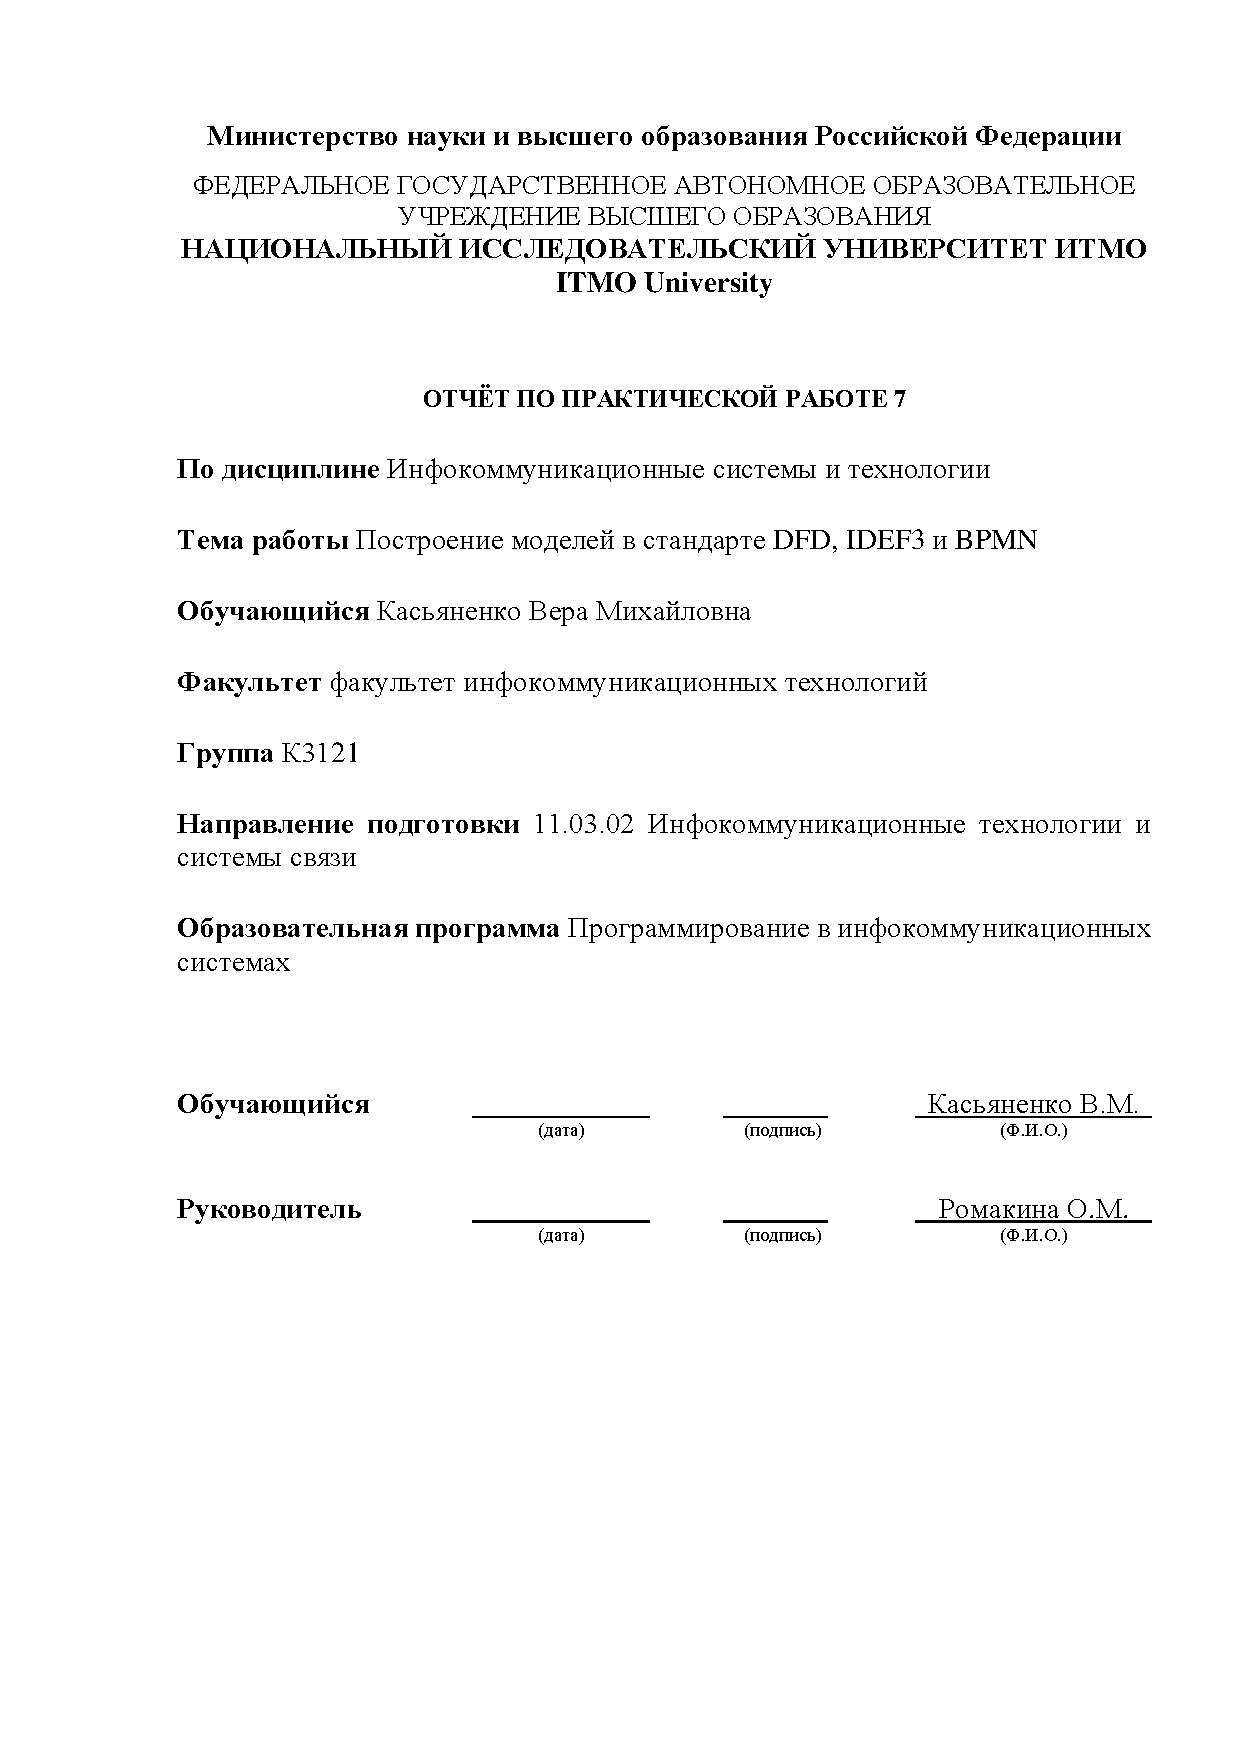
\includepdf[pages=-,pagecommand={}]{titulCourse.pdf}

\pagestyle{plain}
\tableofcontents
 

\intro 

В данном отчете будут представлены диаграммы DFD, модель в стандарте IDEF3, а также модель процесса в стандарте BPMN для мобильного приложения OptiTune.


\chapter{Диаграммы и модели\label{chapter1}}
\section{Диаграммы DFD}

В данном разделе представлены диаграммы DFD. Они представлены как дополнение к диаграмме в стандарте IDEF0. В диаграмму в стандарте IDEF0 входит контекстная диаграмма  (рисунок \ref{fig1}) и декомпозиция этой диаграммы  (рисунок \ref{fig2}). Для этой декомпозиции контекстной диаграммы представлены  декомпозиции блоков "Определение уровня доступа в систему"\ (рисунок \ref{fig3}) и "Обработка запроса пользователя"\ (рисунок \ref{fig4}) в формате DFD.

\begin{landscape}
\begin{figure}[H]
\centerline{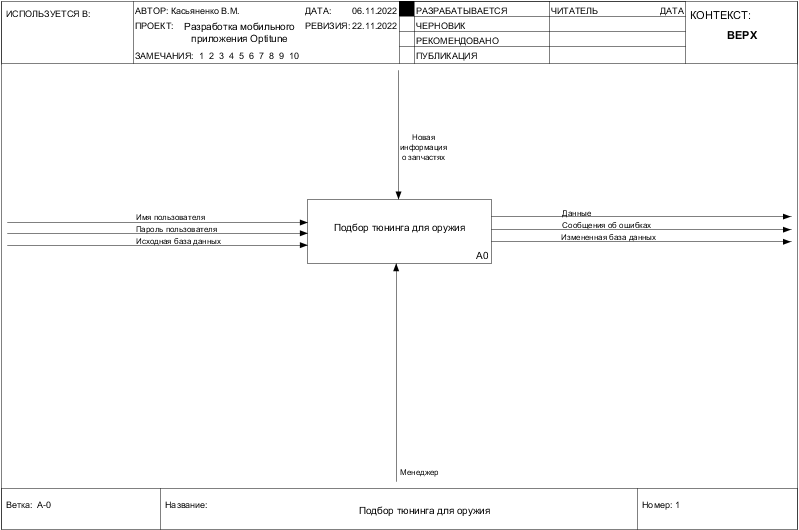
\includegraphics[width=0.9\linewidth]{01_A-0}}
\caption{Контекстная диаграмма в стандарте IDEF0}
\label{fig1}
\end{figure}

\begin{figure}[H]
\centerline{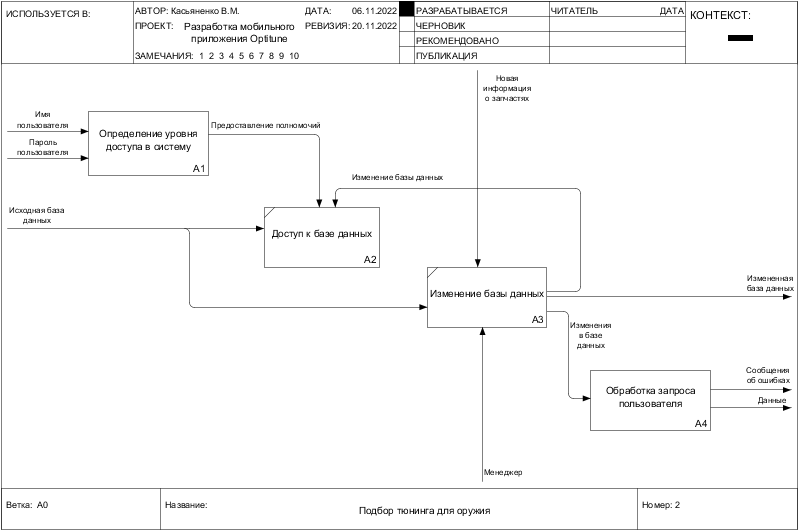
\includegraphics[width=0.9\linewidth]{02_A0}}
\caption{Декомпозиция контекстной диаграммы в стандарте IDEF0}
\label{fig2}
\end{figure}

\begin{figure}[H]
\centerline{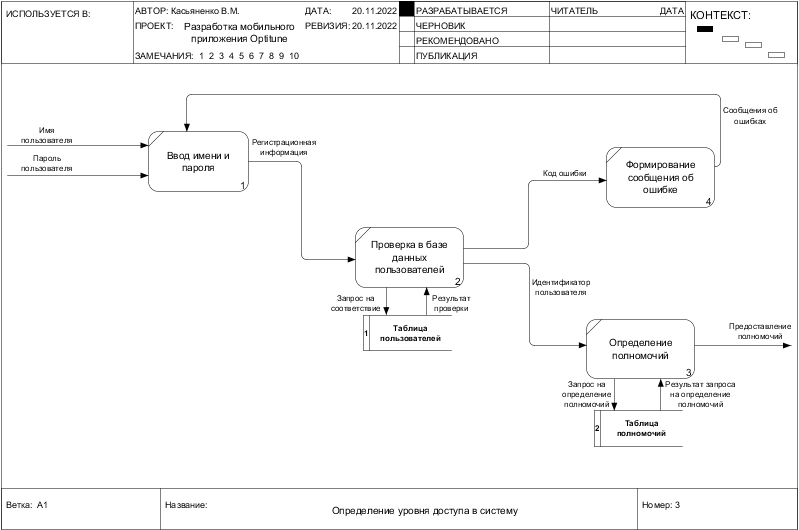
\includegraphics[width=0.9\linewidth]{03_A1}}
\caption{Декомпозиция блока "Определение уровня доступа в систему"\ в стандарте DFD}
\label{fig3}
\end{figure}

\begin{figure}[H]
\centerline{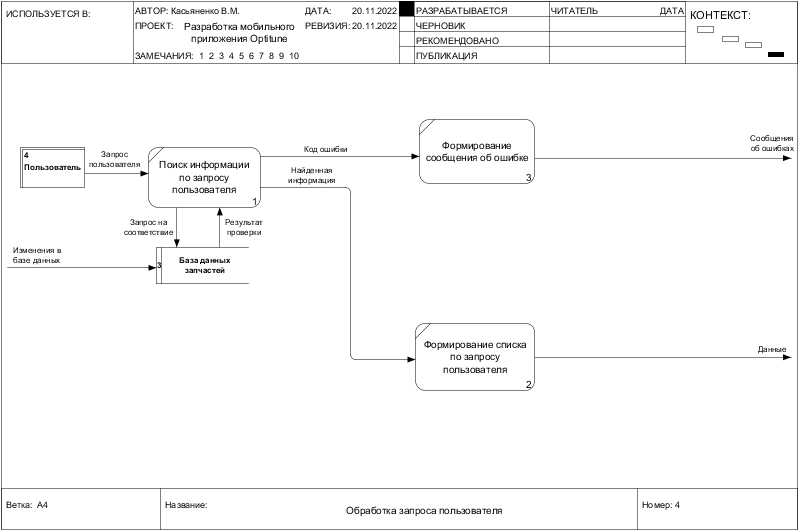
\includegraphics[width=0.9\linewidth]{04_A4}}
\caption{Декомпозиция блока "Обработка запроса пользователя"\ в стандарте DFD}
\label{fig4}
\end{figure}
\end{landscape}

\section{Модель в стандарте IDEF3}

В данном разделе представлена модель в стандарте IDEF3. Она представлены в виде контекстной диаграммы  (рисунок \ref{fig5}) и декомпозиции этой диаграммы  (рисунок \ref{fig6}). Также для декомпозиции контекстной диаграммы представлены декомпозиции блоков "Определение уровня доступа в систему"\ (рисунок \ref{fig7}) и "Обработка запроса пользователя"\ (рисунок \ref{fig8}).

\begin{landscape}
\begin{figure}[H]
\centerline{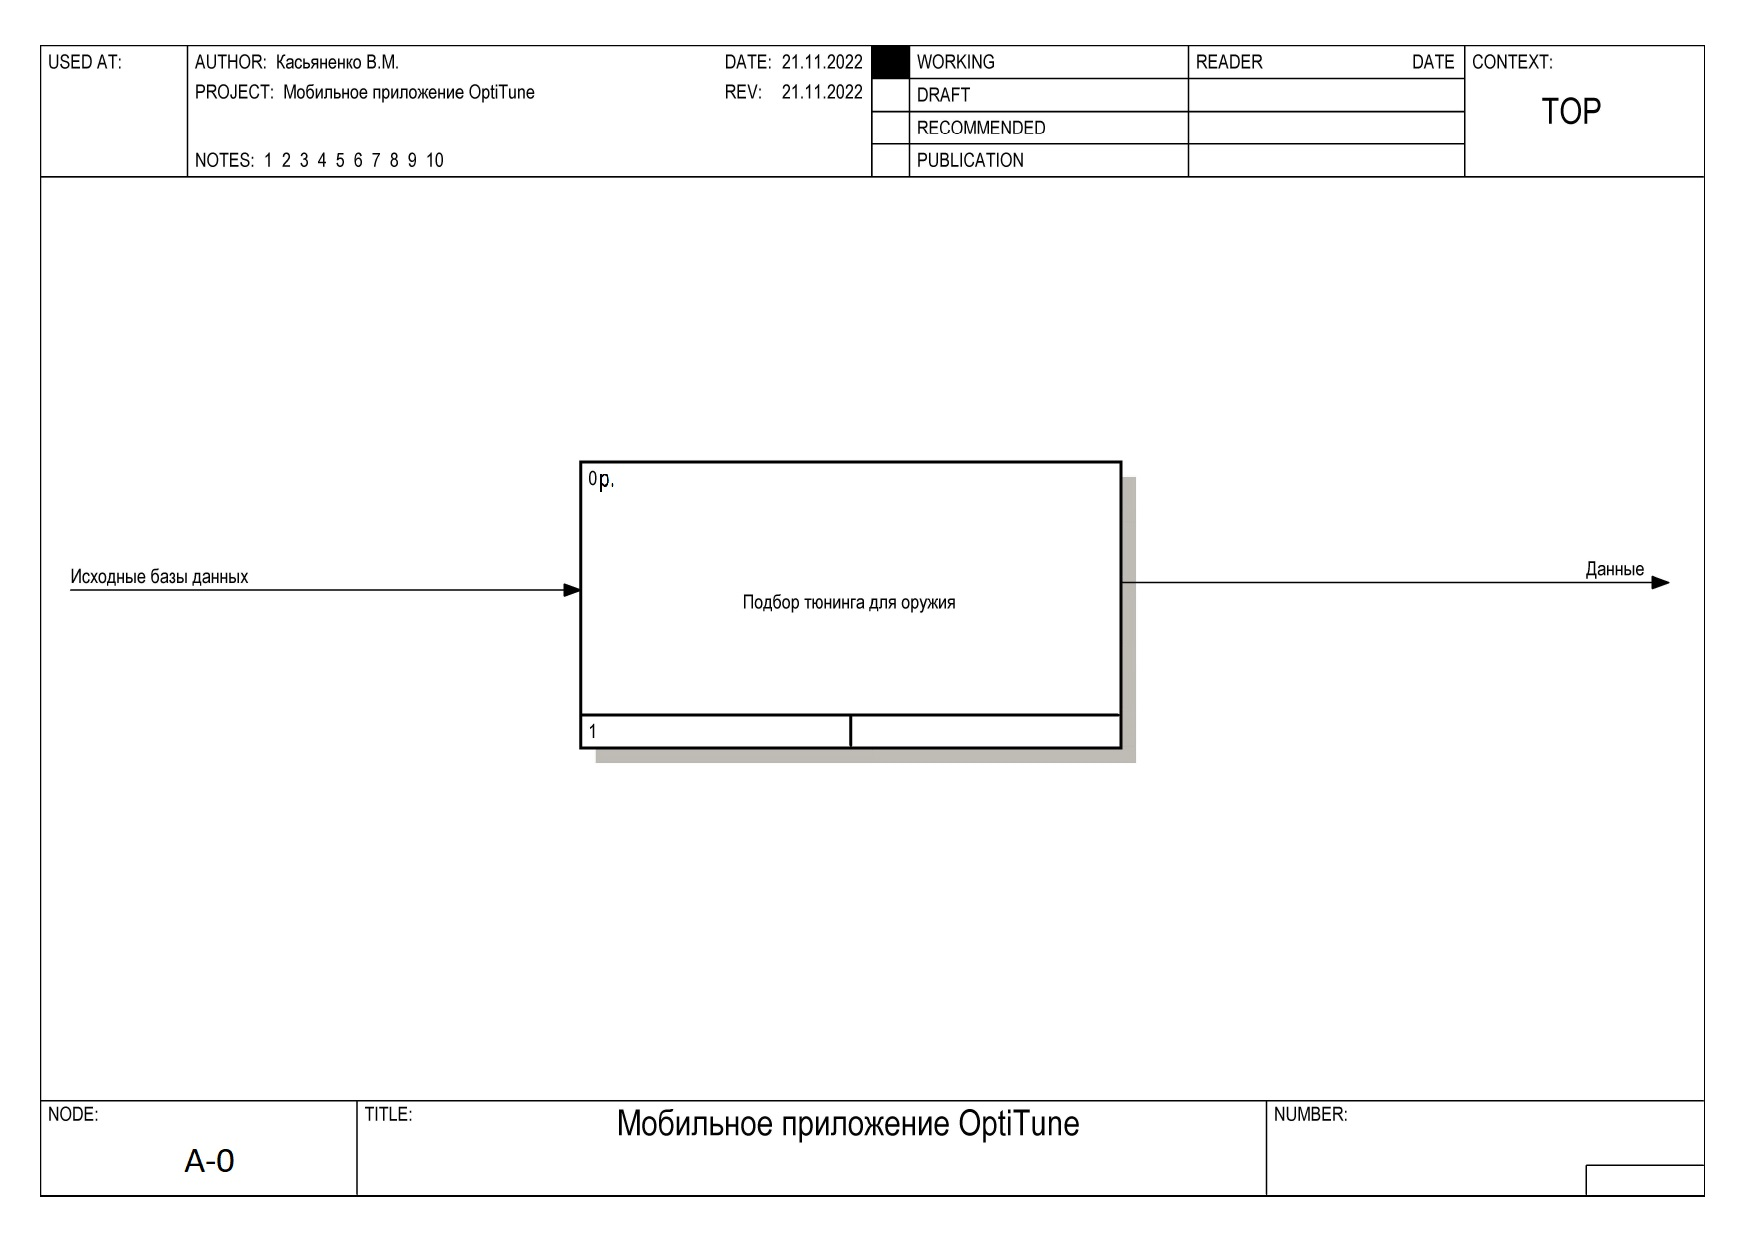
\includegraphics[width=0.9\linewidth]{idef30}}
\caption{Контекстная диаграмма в стандарте IDEF3}
\label{fig5}
\end{figure}

\begin{figure}[H]
\centerline{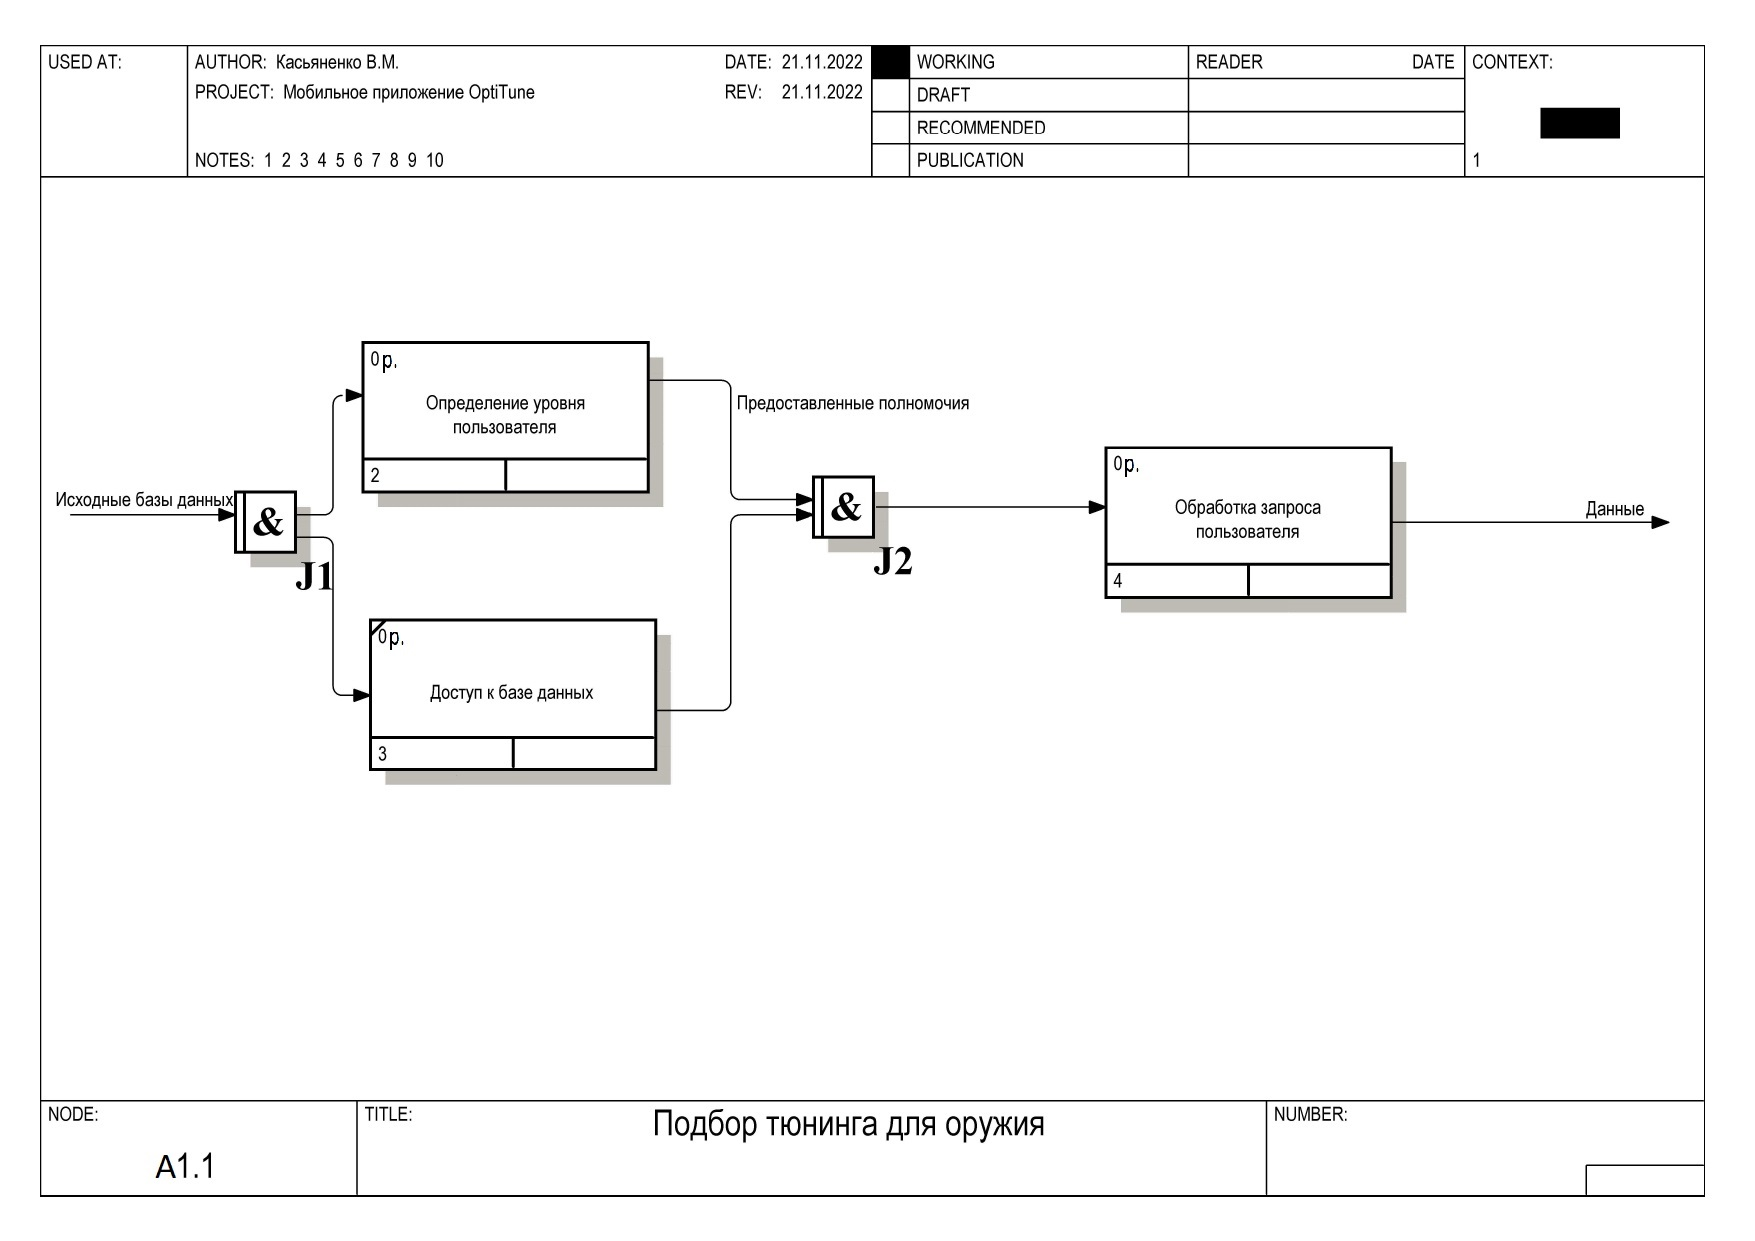
\includegraphics[width=0.9\linewidth]{idef31}}
\caption{Декомпозиция контекстной диаграммы в стандарте IDEF3}
\label{fig6}
\end{figure}

\begin{figure}[H]
\centerline{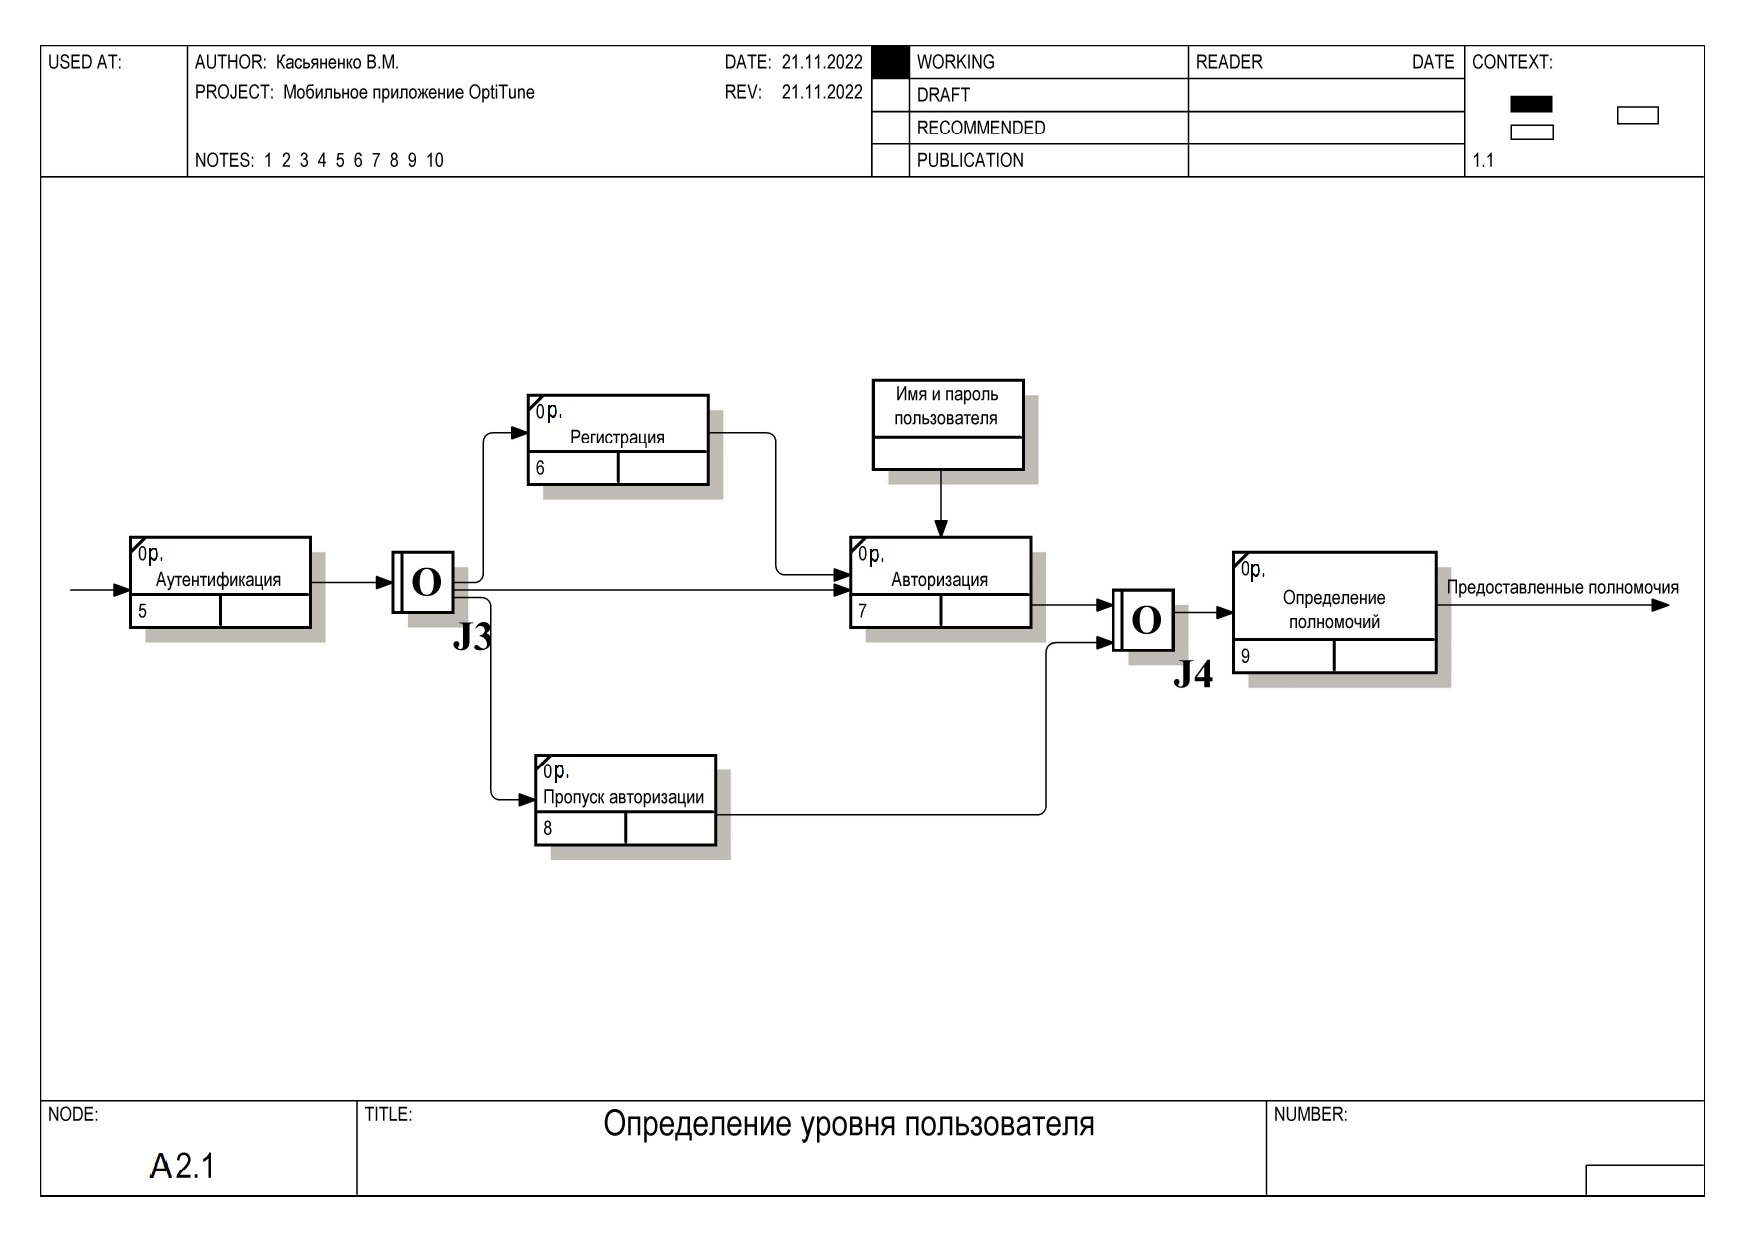
\includegraphics[width=0.9\linewidth]{idef312}}
\caption{Декомпозиция блока "Определение уровня доступа в систему"\ в стандарте IDEF3}
\label{fig7}
\end{figure}

\begin{figure}[H]
\centerline{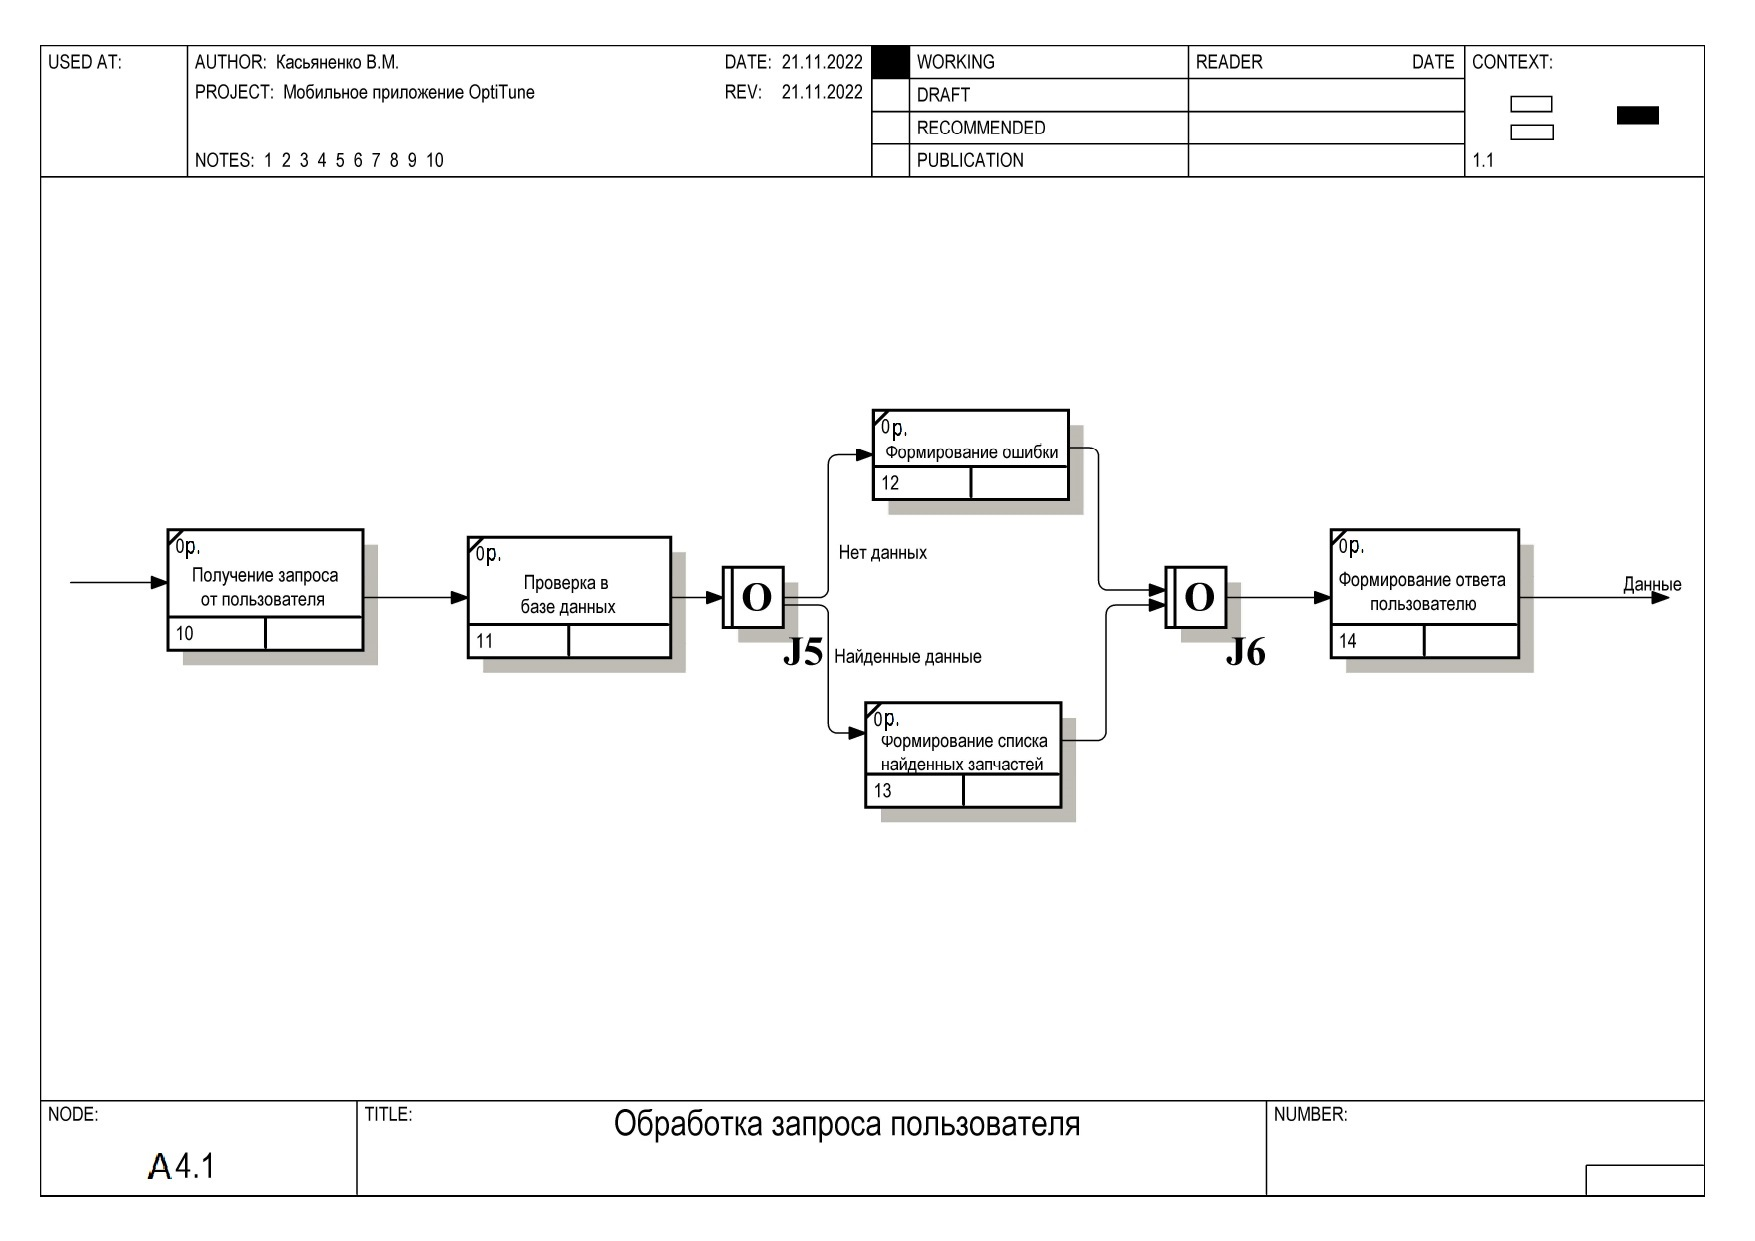
\includegraphics[width=0.9\linewidth]{idef313}}
\caption{Декомпозиция блока "Обработка запроса пользователя"\ в стандарте IDEF3}
\label{fig8}
\end{figure}
\end{landscape}

\section{Модель процесса в нотации BPMN}

В данном разделе представлена модель процесса в нотации BPMN. Она представлены в виде модели процесса  (рисунок \ref{fig9}) и декомпозиции блока "Произвести поиск в базе данных"\  (рисунок \ref{fig10}).

\begin{landscape}
\begin{figure}[H]
\centerline{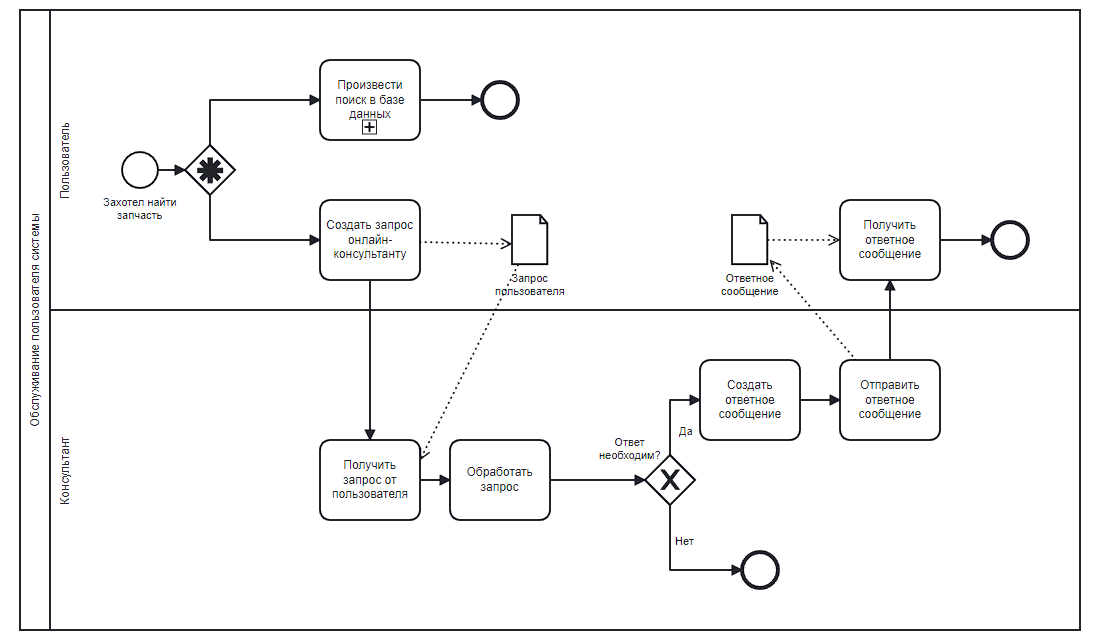
\includegraphics[width=0.9\linewidth]{1}}
\caption{Модель процесса в нотации BPMN}
\label{fig9}
\end{figure}

\begin{figure}[H]
\centerline{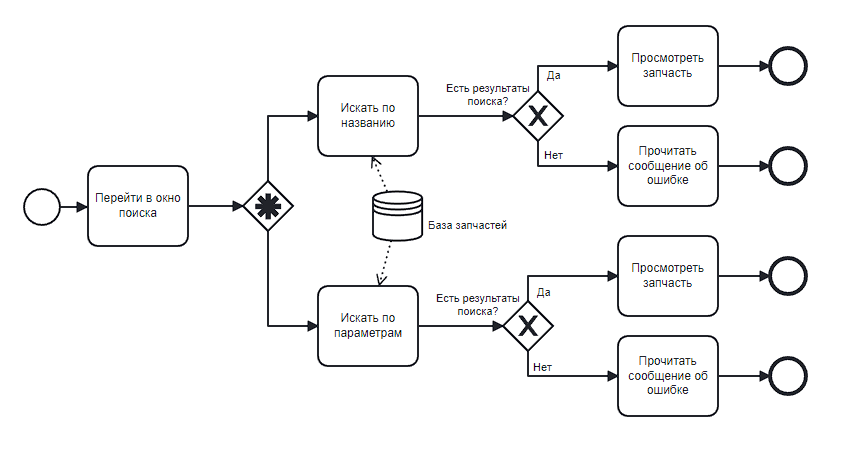
\includegraphics[width=0.9\linewidth]{2}}
\caption{Декомпозиция блока "Произвести поиск в базе данных"\ в нотации BPMN}
\label{fig10}
\end{figure}
\end{landscape}

\conclusions

Был составлен отчет, в котором были представлены диаграммы DFD, модель в стандарте IDEF3, а также модель процесса в стандарте BPMN для мобильного приложения OptiTune.


\newpage
\begin{thebibliography}{99}

\bibitem{bib1} Wikipedia: официальный сайт. – URL: \url{https://ru.wikipedia.org/wiki/BPMN} (Дата обращения 21.11.2022).

\end{thebibliography}

\end{document}